\documentclass[border=0pt]{standalone}
\usepackage{fontspec}
\usepackage{tikz}
\usetikzlibrary{arrows.meta,positioning,backgrounds,fit,calc}

\definecolor{ink}{HTML}{1E293B}
\definecolor{sub}{HTML}{64748B}
\definecolor{page}{HTML}{FFFFFF}
\definecolor{card}{HTML}{F8FAFC}
\definecolor{line}{HTML}{CBD5E1}
\definecolor{on}{HTML}{059669}      % emerald: Tor ON
\definecolor{off}{HTML}{64748B}     % slate: Tor OFF
\definecolor{app}{HTML}{2563EB}

\newcommand{\hd}[1]{{\bfseries #1}}
\newcommand{\subt}[1]{{\scriptsize\color{sub} #1}}

\pgfdeclarelayer{bg}\pgfdeclarelayer{bg2}\pgfsetlayers{bg2,bg,main}

\begin{document}
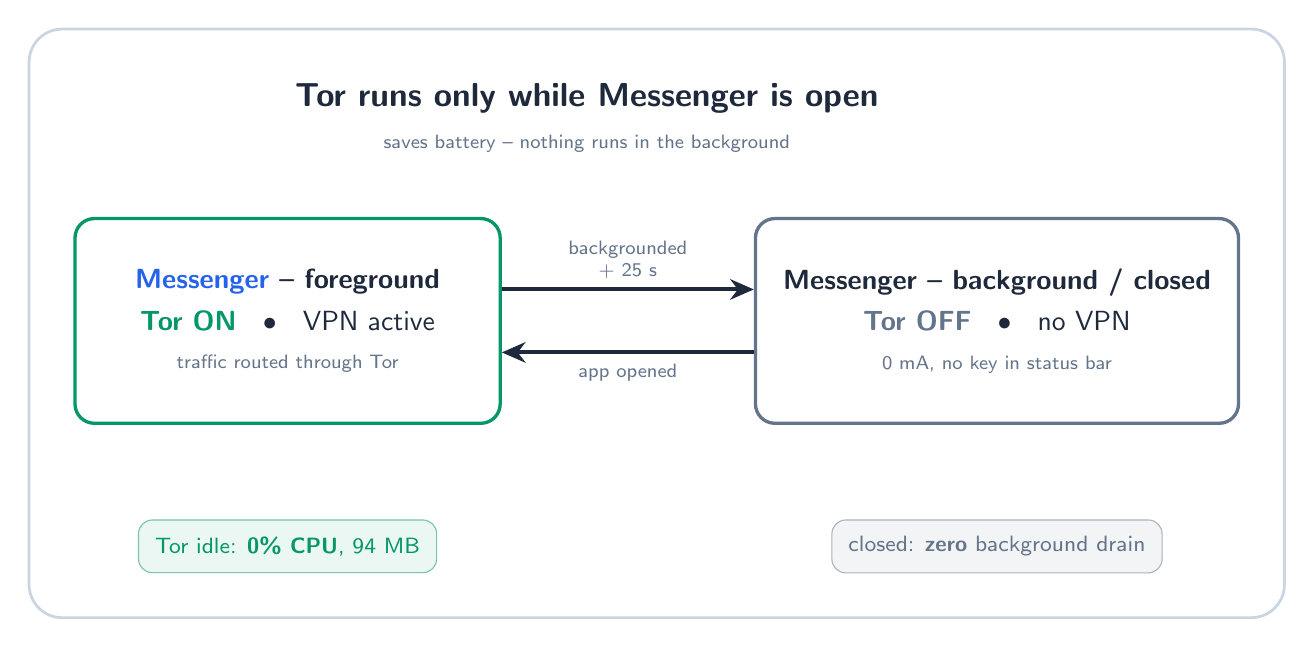
\begin{tikzpicture}[
  font=\sffamily,
  state/.style={rounded corners=7pt, draw=#1, line width=1.2pt, fill=white, text=ink,
                align=center, inner sep=10pt, minimum width=54mm, minimum height=26mm},
  sublbl/.style={font=\sffamily\scriptsize, text=sub},
  tr/.style={-{Stealth[length=3mm,width=2.6mm]}, line width=1.4pt, draw=ink},
  fact/.style={rounded corners=5pt, draw=#1!55, fill=#1!8, text=#1,
               font=\sffamily\footnotesize, inner sep=6pt, align=center},
]

% title
\node[font=\sffamily\large\bfseries, text=ink] (h1)
  {Tor runs only while Messenger is open};
\node[sublbl, below=1pt of h1] (h2) {saves battery -- nothing runs in the background};

% two states
\node[state=on, below=12mm of h1.south, xshift=-38mm] (on) {%
  \hd{\textcolor{app}{Messenger} -- foreground}\\[3pt]
  \textcolor{on}{\hd{Tor ON}} \; $\bullet$ \; VPN active\\[2pt]
  \subt{traffic routed through Tor}};
\node[state=off, right=32mm of on] (off) {%
  \hd{Messenger -- background / closed}\\[3pt]
  \textcolor{off}{\hd{Tor OFF}} \; $\bullet$ \; no VPN\\[2pt]
  \subt{0 mA, no key in status bar}};

% transitions
\draw[tr] ([yshift=4mm]on.east) -- node[above, sublbl, align=center]{backgrounded\\ + 25 s} ([yshift=4mm]off.west);
\draw[tr] ([yshift=-4mm]off.west) -- node[below, sublbl]{app opened} ([yshift=-4mm]on.east);

% facts strip
\node[fact=on,  below=12mm of on.south]  (f1) {Tor idle: \hd{0\% CPU}, 94 MB};
\node[fact=off, below=12mm of off.south] (f2) {closed: \hd{zero} background drain};

% background card
\begin{pgfonlayer}{bg2}
  \node[fill=page, draw=line, line width=1pt, rounded corners=12pt,
        fit=(h1)(h2)(on)(off)(f1)(f2), inner sep=16pt] {};
\end{pgfonlayer}
\end{tikzpicture}
\end{document}
